\documentclass[conference]{IEEEtran}

\usepackage[utf8]{inputenc}
\usepackage[T1]{fontenc}
\usepackage[spanish,es-noshorthands,es-tabla]{babel}
\usepackage{amsmath,amssymb}
\usepackage{graphicx}
\usepackage{booktabs}
\usepackage{tikz}
\usetikzlibrary{positioning,arrows.meta}

\graphicspath{{figures/}}

% evita que los nombres largos de funciones se salgan de la columna
\emergencystretch=1.5em

% COMPLETAR: altura del peluche medida con regla (mm) y el error relativo
\newcommand{\alturareal}{\textbf{[COMPLETAR]}}
\newcommand{\errorrel}{\textbf{[COMPLETAR]}}

\begin{document}

\title{Reconstrucción 3D de un objeto mediante visión estéreo multivista}

\author{\IEEEauthorblockN{Pedro Beresten, Camila Di Paola, Maria Victoria Persico, Sofia Yabo}
\IEEEauthorblockA{Universidad de San Andrés\\
Visión Artificial\\
Semestre Primavera 2026\\
Profesor: Gastón Castro}}

\maketitle

% =====================================================================
\section{Introducción y marco teórico}
% =====================================================================

El objetivo del trabajo es reconstruir la nube de puntos 3D de un objeto
(un peluche) a partir de múltiples pares de imágenes tomadas con una cámara
estéreo, y estimar sus dimensiones reales en milímetros. Para ello se
implementó un pipeline de fotogrametría estéreo multivista: calibración del
sistema, rectificación, cálculo de disparidad, reconstrucción de una nube
local por cada par, estimación de la pose de la cámara respecto de un objeto
de referencia conocido (un tablero ChArUco), fusión de todas las nubes en un
marco común y optimización de la nube final. A continuación se resumen los
conceptos en los que se apoya cada etapa.

\subsection{Modelo de cámara pinhole y distorsión}

El modelo pinhole describe la formación de la imagen como una proyección
central: un punto del mundo $\mathbf{X}_w=(X,Y,Z)^\top$ se lleva primero al
sistema de la cámara mediante una transformación rígida y luego se proyecta
sobre el plano imagen,
\begin{equation}
  s\begin{pmatrix}u\\v\\1\end{pmatrix}
  = K\,[R\,|\,\mathbf{t}]
  \begin{pmatrix}\mathbf{X}_w\\1\end{pmatrix},
  \label{eq:pinhole}
\end{equation}
\begin{equation}
  K=\begin{pmatrix} f_x & 0 & c_x\\ 0 & f_y & c_y\\ 0&0&1\end{pmatrix},
\end{equation}
donde $s$ es un factor de escala (la profundidad del punto). La matriz $K$
contiene los \emph{parámetros intrínsecos}: las distancias focales $f_x, f_y$
expresadas en píxeles y el punto principal $(c_x, c_y)$, donde el eje óptico
corta al sensor. $R$ y $\mathbf{t}$ son los \emph{parámetros extrínsecos}, que
indican la pose de la cámara respecto del mundo.

Las lentes reales, y en particular las gran angulares como las de la cámara
utilizada, se apartan de este modelo ideal. La distorsión se modela sobre las
coordenadas normalizadas $(x,y)$, con $r^2=x^2+y^2$, mediante una componente
radial ($k_1,k_2,k_3$) y una tangencial ($p_1,p_2$). Con
$L(r)=1+k_1r^2+k_2r^4+k_3r^6$,
\begin{align}
  x_d &= x\,L(r) + 2p_1xy + p_2(r^2+2x^2),\\
  y_d &= y\,L(r) + p_1(r^2+2y^2) + 2p_2xy.
\end{align}

Calibrar consiste en estimar $K$ y los coeficientes de distorsión. Es
necesario porque, sin conocerlos, no es posible relacionar un píxel con el
rayo 3D que lo generó: no se podría corregir la distorsión, rectificar el par
estéreo ni convertir disparidades en distancias métricas.

\subsection{Calibración estéreo y error de reproyección}

La calibración se realiza con el método de Zhang: se fotografía desde muchas
vistas un patrón plano de geometría conocida (un \emph{checkerboard}), cuyos
puntos $\mathbf{M}_j$ tienen coordenadas exactas en milímetros sobre el plano
$Z=0$. Para cada vista $i$ se detectan sus esquinas $\mathbf{m}_{ij}$ con
precisión subpíxel y se estiman los parámetros minimizando el error de
reproyección mediante optimización no lineal (Levenberg--Marquardt):
\begin{equation}
  \min_{K,\,D,\,\{R_i,\mathbf{t}_i\}}\;
  \sum_{i}\sum_{j}\bigl\|\mathbf{m}_{ij}-\pi_i(\mathbf{M}_j)\bigr\|^2,
\end{equation}
donde $\pi_i$ es la proyección de la ecuación~\eqref{eq:pinhole} con
distorsión, usando $K$, $D$ y la pose $(R_i,\mathbf{t}_i)$ de la vista $i$.

En un sistema estéreo, además de los intrínsecos de cada cámara, se estiman
los \emph{extrínsecos relativos} $(R, T)$ que llevan puntos del sistema de la
cámara izquierda al de la derecha:
$\mathbf{X}_R = R\,\mathbf{X}_L + T$. Como ambas cámaras observan el mismo
tablero simultáneamente, en cada vista se cumple $R_{R,i}=R\,R_{L,i}$ y
$\mathbf{t}_{R,i}=R\,\mathbf{t}_{L,i}+T$, y \texttt{cv2.stereoCalibrate}
optimiza conjuntamente todos los parámetros con esa restricción. La norma
$\|T\|$ es el \emph{baseline}, la distancia entre los centros ópticos, y queda
en milímetros porque el tamaño del cuadrado del tablero se especifica en
milímetros. A partir de $(R,T)$ se obtienen la matriz esencial
$E=[T]_\times R$ y la fundamental $F=K_R^{-\top}EK_L^{-1}$, que codifican la
geometría epipolar del par.

El \emph{error de reproyección} es la distancia, en píxeles, entre la posición
detectada de cada esquina y la posición en la que el modelo calibrado la
proyecta. Se reporta como su valor cuadrático medio,
\begin{equation}
  \mathrm{RMS}=\sqrt{\frac{1}{N}\sum_{i,j}\bigl\|\mathbf{m}_{ij}-\hat{\mathbf{m}}_{ij}\bigr\|^2},
\end{equation}
y es la principal medida de calidad de la calibración: valores del orden de
1~píxel o menos indican que el modelo explica bien las observaciones.

\subsection{Geometría epipolar y rectificación}

Dado un punto $\mathbf{x}_L$ en la imagen izquierda, su correspondiente en la
imagen derecha no puede estar en cualquier lugar: debe estar sobre la
\emph{línea epipolar} $\mathbf{l}_R=F\mathbf{x}_L$, ya que se cumple la
restricción $\mathbf{x}_R^\top F\,\mathbf{x}_L=0$. Esto reduce la búsqueda de
correspondencias de dos dimensiones a una. Sin embargo, en general las
líneas epipolares son oblicuas y distintas para cada punto, lo que hace la
búsqueda costosa.

La \emph{rectificación estéreo} aplica a cada imagen una rotación virtual
($R_1$, $R_2$) y una nueva matriz de proyección ($P_1$, $P_2$), de modo que
ambos planos imagen queden coplanares y paralelos al baseline, con la misma
distancia focal. Junto con la corrección de la distorsión, esto se condensa
en mapas de remapeo píxel a píxel (\texttt{cv2.initUndistortRectifyMap} y
\texttt{cv2.remap}). En el par rectificado todas las líneas epipolares son
horizontales y coinciden entre imágenes: el correspondiente de un píxel
$(x,y)$ de la izquierda está en la \emph{misma fila} $y$ de la derecha. Así el
\emph{matching} se convierte en una búsqueda unidimensional sobre una fila,
mucho más rápida y robusta, y la diferencia de posiciones se reduce a un
único número por píxel: la disparidad.

\subsection{De disparidad a profundidad}

En un par rectificado con distancia focal $f$ (en píxeles) y baseline $B$,
la disparidad de un punto es $d=x_L-x_R$. Por semejanza de triángulos,
\begin{align}
  Z &= \frac{f\,B}{d}, \label{eq:depth}\\
  X &= \frac{(x_L-c_x)\,Z}{f},\qquad
  Y = \frac{(y-c_y)\,Z}{f}.
\end{align}
La profundidad es inversamente proporcional a la disparidad: los objetos
cercanos tienen disparidades grandes. \texttt{cv2.stereoRectify} devuelve una
matriz $Q$ de $4\times4$ que resume estas relaciones en coordenadas
homogéneas, $(X,Y,Z,W)^\top=Q\,(x,y,d,1)^\top$, y que
\texttt{cv2.reprojectImageTo3D} aplica a todo el mapa de disparidad.

Derivando la ecuación~\eqref{eq:depth} se obtiene
\begin{equation}
  |\Delta Z|\approx \frac{Z^2}{fB}\,|\Delta d|,
  \label{eq:dz}
\end{equation}
es decir, el error en profundidad crece con el cuadrado de la distancia. Con
$f\approx600$~px y $B\approx61$~mm, un error de medio píxel en la disparidad
implica unos 2~mm de error a 40~cm, pero unos 9~mm a 80~cm. Por eso conviene
capturar el objeto de cerca.

\subsection{Pose de la cámara con PnP}

Cada nube obtenida con $Q$ está expresada en el sistema de la cámara
izquierda de esa captura, que cambia de una toma a otra. Para fusionarlas es
necesario conocer la pose de la cámara respecto de un marco fijo (el
``mundo''), que en este trabajo es un tablero ChArUco apoyado debajo del
objeto. Conocidas las coordenadas 3D $\mathbf{M}_j$ de puntos del tablero y
sus proyecciones $\mathbf{m}_j$ en la imagen, el problema
\emph{Perspective-n-Point} (PnP) consiste en encontrar $(R,\mathbf{t})$ que
minimizan el error de reproyección con $K$ conocida.
\texttt{cv2.solvePnP} devuelve la rotación como un \emph{vector de Rodrigues}
$\mathbf{r}=\theta\,\mathbf{k}$, cuya dirección $\mathbf{k}$ es el eje de
giro y cuya norma $\theta$ es el ángulo. \texttt{cv2.Rodrigues} lo convierte
en matriz:
\begin{equation}
  R = I + \sin\theta\,[\mathbf{k}]_\times + (1-\cos\theta)\,[\mathbf{k}]_\times^2 .
\end{equation}
La pose obtenida lleva puntos del mundo a la cámara,
$\mathbf{X}_c=R\,\mathbf{X}_w+\mathbf{t}$; para llevar la nube local al
mundo se usa la inversa,
\begin{equation}
  \mathbf{X}_w = R^\top(\mathbf{X}_c-\mathbf{t}).
  \label{eq:cam2world}
\end{equation}

\subsection{Por qué la reconstrucción es métrica}

Una reconstrucción a partir de imágenes de una sola cámara en movimiento
solo puede recuperarse salvo un factor de escala desconocido. En este caso,
en cambio, la escala queda fijada por dos medidas físicas: el baseline $B$,
estimado en milímetros gracias al tamaño conocido del cuadrado del
checkerboard de calibración, y el tamaño conocido de los cuadrados del
ChArUco, que hace que la traslación de cada pose esté en milímetros. Por lo
tanto, las coordenadas de la nube fusionada están directamente en milímetros
y las distancias medidas sobre ella son dimensiones reales.

% =====================================================================
\section{Metodología}
% =====================================================================

El pipeline se implementó en Python con OpenCV~4.13 y Open3D~0.19
(directorio \texttt{pipeline/} del repositorio). El script
\texttt{run\_pipeline.py} ejecuta todas las etapas a partir de un archivo de
configuración YAML. La Figura~\ref{fig:pipeline} resume el flujo.

\begin{figure*}[t]
  \centering
  \begin{tikzpicture}[
      node distance=4mm,
      box/.style={draw, rounded corners, align=center, font=\small,
                  minimum height=10mm, text width=21mm},
      arr/.style={-{Latex[length=2mm]}}]
    \node[box] (cal) {Calibración\\estéreo};
    \node[box, right=of cal] (rect) {Rectificación};
    \node[box, right=of rect] (disp) {Disparidad\\(CREStereo)};
    \node[box, right=of disp] (nube) {Nube local\\($Q$)};
    \node[box, below=8mm of nube] (pose) {Pose\\(ChArUco+PnP)};
    \node[box, left=of pose] (fus) {Fusión en el\\mundo};
    \node[box, left=of fus] (opt) {Optimización};
    \node[box, left=of opt] (med) {Medición\\y \texttt{.ply}};
    \draw[arr] (cal) -- (rect);
    \draw[arr] (rect) -- (disp);
    \draw[arr] (disp) -- (nube);
    \draw[arr] (nube) -- (pose);
    \draw[arr] (pose) -- (fus);
    \draw[arr] (fus) -- (opt);
    \draw[arr] (opt) -- (med);
  \end{tikzpicture}
  \caption{Etapas del pipeline de reconstrucción. Las etapas de disparidad,
  nube local y pose se repiten para cada uno de los 58 pares de captura.}
  \label{fig:pipeline}
\end{figure*}

\subsection{Dataset}

Las imágenes se capturaron con la cámara estéreo ELP-USB3D1080P02-H120
(1920$\times$1080 píxeles por cámara) usando la herramienta
\texttt{calib-stereo} de la cátedra. Se generaron dos colecciones:
\begin{itemize}
  \item \textbf{Calibración:} 81 pares de un checkerboard de 9$\times$6
        esquinas internas con cuadrados de 28~mm, en distintas distancias,
        inclinaciones y posiciones dentro del campo visual.
  \item \textbf{Reconstrucción:} 58 pares del peluche apoyado sobre un
        tablero ChArUco de 9$\times$13 cuadrados (diccionario
        \texttt{DICT\_5X5\_100}, cuadrados de 42~mm y marcadores de
        31.5~mm), tomados recorriendo el objeto a su alrededor sin moverlo
        respecto del tablero.
\end{itemize}

\subsection{Calibración y rectificación}

Si bien la herramienta de la cátedra ya genera los archivos de calibración,
se reimplementó la calibración con funciones de OpenCV para poder reportar el
error de reproyección y el error por vista. En cada par se detecta el
checkerboard con \texttt{cv2.findChessboardCorners} y se refinan las esquinas
con \texttt{cv2.cornerSubPix}; se descartan los pares en los que no se
detecta en ambas imágenes. Los puntos 3D del tablero se generan sobre el
plano $Z=0$ escalados por el tamaño del cuadrado (28~mm), de modo que la
calibración queda en milímetros. Luego se estiman conjuntamente los
intrínsecos, la distorsión y los extrínsecos relativos con
\texttt{cv2.stereoCalibrate}\allowbreak\texttt{Extended} (variante de
\texttt{stereoCalibrate} que además devuelve el error por vista). Los
resultados coinciden con los obtenidos por la herramienta
\texttt{calib-stereo}.

Para la rectificación se usó \texttt{cv2.stereoRectify} con
\texttt{alpha=0}, que recorta la imagen rectificada para que no queden zonas
negras sin información, y \texttt{cv2.initUndistortRectifyMap} para construir
los mapas que luego se aplican a cada par con \texttt{cv2.remap}. De esta
etapa se obtienen también $R_1$, $P_1$ y la matriz $Q$ usadas más adelante.

\subsection{Disparidad y nube local}

Se probaron dos métodos de \emph{stereo matching} sobre los pares
rectificados:
\begin{itemize}
  \item \textbf{StereoSGBM} (OpenCV), que combina un costo de matching por
        bloques con una regularización semi-global que penaliza los cambios
        de disparidad entre píxeles vecinos (penalizaciones
        $P_1=8b^2$ y $P_2=32b^2$, con $b$ el tamaño de bloque).
        Se usó el modo \texttt{3WAY}, bloque de $b=5$,
        \texttt{uniquenessRatio}~$=10$ y filtrado de \emph{speckles}
        (ventana 200, rango 2). El número de disparidades se fijó en 192 a
        partir de la ecuación~\eqref{eq:depth}: con $f\approx600$~px y
        $B\approx61$~mm, el objeto a 25~cm produce disparidades de unos
        145~px y a 80~cm de unos 45~px.
  \item \textbf{CREStereo}, una red neuronal recurrente en cascada para
        estéreo (CVPR 2022), usando el módulo \texttt{disparity} provisto por
        la cátedra. La red trabaja a 1280$\times$720 con 10 iteraciones de
        refinamiento, y la disparidad se reescala a la resolución original.
\end{itemize}
Con SGBM solo alrededor del 50\% de los píxeles obtenían una disparidad
válida y la superficie del tablero resultaba muy ruidosa, en buena parte por
las zonas de poca textura del peluche y por el desalineamiento vertical
residual entre imágenes que se analiza en la Discusión. CREStereo produjo
mapas densos y mucho más limpios, por lo que se eligió para la reconstrucción
final (unos 15~s por par en CPU; los resultados se guardan en caché).

A partir de la disparidad se calcula la nube local con
\texttt{cv2.reprojectImageTo3D} y la matriz $Q$. Se descartan los píxeles con
disparidad no válida y los puntos fuera del rango de profundidad
$100<Z<1000$~mm, que no pueden corresponder a la escena de interés. A cada
punto se le asigna el color del píxel de la imagen izquierda rectificada. La
nube resultante está expresada en el sistema de la cámara izquierda
\emph{rectificada}.

\subsection{Pose de la cámara y paso al marco global}

Para cada captura se detecta el ChArUco en la imagen izquierda con
\texttt{cv2.aruco.CharucoDetector}. Como el peluche tapa buena parte del
tablero, en muchas vistas se interpolan pocas esquinas ChArUco, por lo que
como correspondencias 2D--3D se usan tanto las esquinas ChArUco interpoladas
como las cuatro esquinas de cada marcador ArUco detectado, cuyas coordenadas
en el tablero se conocen.

Un detalle importante es en qué sistema se estima la pose. La nube local está
en el sistema de la cámara izquierda rectificada, que difiere del sistema
original por la rotación $R_1$. Para evitar tener que componer con $R_1$, la
pose se estima directamente sobre la imagen izquierda \emph{rectificada},
usando como intrínseca $K_{\text{rect}}=P_1[:, :3]$ y distorsión nula (la
distorsión ya fue corregida por el remapeo). Así, la pose y la nube quedan
exactamente en el mismo sistema de referencia.

Dado que todos los puntos de correspondencia son coplanares, la estimación
inicial se calcula con \texttt{cv2.solvePnP} usando el método
\texttt{SOLVEPNP\_IPPE}, específico para patrones planos, y luego se refina
con \texttt{cv2.solvePnPRefineLM}, que minimiza el error de reproyección por
Levenberg--Marquardt. El vector de Rodrigues se convierte en matriz con
\texttt{cv2.Rodrigues} y se arma la transformación homogénea cámara$\to$mundo
de la ecuación~\eqref{eq:cam2world},
\begin{equation}
  T_{wc}=\begin{pmatrix} R^\top & -R^\top\mathbf{t}\\ \mathbf{0}^\top & 1\end{pmatrix}.
\end{equation}
En el marco del tablero que usa OpenCV el eje $Z$ apunta hacia adentro del
tablero, por lo que se aplica además una rotación de $180^\circ$ alrededor de
$X$, $\mathrm{diag}(1,-1,-1)$, para que el eje $Z$ del mundo apunte hacia
arriba y la altura del objeto sea directamente su coordenada $Z$. Para
verificar las poses se calculó el error de reproyección de PnP en cada
captura y se visualizaron las cámaras como pirámides junto con los ejes del
mundo, comprobando que reproducen la trayectoria de captura alrededor del
objeto.

\subsection{Fusión y optimización de la nube}

Las 58 nubes locales se transforman al mundo con su $T_{wc}$ y se concatenan
en una única nube, que contiene unos 100 millones de puntos y toda la escena.
Sobre ella se aplican en Open3D los siguientes pasos:
\begin{enumerate}
  \item \textbf{Filtrado espacial:} se define en coordenadas del mundo una
        caja que encierra al peluche
        ($140\le X\le370$, $-450\le Y\le-160$, $-20\le Z\le250$~mm) y se
        descartan los puntos externos con \texttt{OrientedBoundingBox},
        \texttt{get\_point\_indices\_}\allowbreak\texttt{within\_bounding\_box}
        y \texttt{select\_by\_index}. Como el mundo está alineado al tablero,
        la caja se definió alineada a sus ejes. El límite inferior negativo
        deja dentro una porción del tablero, necesaria para el paso~3.
  \item \textbf{Submuestreo:} \texttt{voxel\_down\_sample} con vóxeles de
        1~mm, que unifica los puntos redundantes provenientes de distintas
        vistas manteniendo un nivel de detalle suficiente para un objeto de
        este tamaño.
  \item \textbf{Remoción del plano de apoyo:} se ajusta por RANSAC
        (\texttt{segment\_plane}, umbral de 3~mm, 2000 iteraciones) el plano
        del tablero reconstruido y se eliminan los puntos a menos de 15~mm de
        él. El margen es mayor que el ruido típico porque el tablero
        reconstruido presenta un espesor de 1 a 4~cm.
  \item \textbf{Eliminación de outliers:}
        \texttt{remove\_statistical\_}\allowbreak\texttt{outlier} con 30
        vecinos y \texttt{std\_ratio}~$=1.5$: para cada punto se calcula la
        distancia media a sus 30 vecinos más cercanos y se descartan los
        puntos en los que esa distancia supera la media global en más de
        1.5 desvíos estándar (puntos aislados).
  \item \textbf{Componente principal:} agrupamiento DBSCAN
        (\texttt{cluster\_dbscan}, $\varepsilon=5$~mm, mínimo 20 puntos),
        conservando solo el cluster más grande, para eliminar los restos del
        tablero y los objetos espurios que quedaron \emph{separados} del
        peluche después de los pasos anteriores.
\end{enumerate}
En cada etapa se registra la cantidad de puntos sobrevivientes. La nube final
se exporta en formato PLY binario con
\texttt{o3d.io.write\_point\_cloud}.

Como paso opcional se generó además una malla: se estiman las normales
(\texttt{estimate\_normals}, radio de 5~mm) y se orientan de forma
consistente, se aplica la reconstrucción de Poisson con profundidad de octree
8, se eliminan el 5\% de los vértices con menor densidad de puntos de soporte
(donde Poisson ``inventa'' superficie) y se simplifica la malla a 200\,000
triángulos.

\subsection{Medición métrica}

Como la nube está en milímetros y en un marco alineado al tablero, la altura
del objeto se mide como la distancia de sus puntos al plano de apoyo
estimado por RANSAC. Para que un punto espurio aislado no infle la medida, se
toma el percentil 99.5 de esas distancias en lugar del máximo. El ancho y la
profundidad se miden como la extensión de la nube en los ejes $X$ e $Y$ del
mundo, entre los percentiles 0.5 y 99.5. Finalmente, la altura estimada se
compara con la medida del peluche tomada con una regla.

% =====================================================================
\section{Resultados}
% =====================================================================

\subsection{Calibración y rectificación}

El checkerboard se detectó en los 81 pares de calibración. La
Tabla~\ref{tab:calib} resume los parámetros obtenidos. El error RMS estéreo
fue de 1.07~px y el baseline de 60.70~mm. Los coeficientes de distorsión son
chicos porque el modelo se ajusta en coordenadas normalizadas; aun así, la
corrección es visible en los bordes de la imagen gran angular. La rotación
relativa entre cámaras es de apenas $0.96^\circ$, es decir, las dos cámaras
están casi alineadas, como corresponde a un módulo estéreo de fábrica.

\begin{table}[t]
  \centering
  \caption{Parámetros de la calibración estéreo (dataset propio).}
  \label{tab:calib}
  \begin{tabular}{@{}lcc@{}}
    \toprule
    & Izquierda & Derecha \\
    \midrule
    $f_x,\ f_y$ [px] & 604.5,\ 602.1 & 605.7,\ 603.0 \\
    $c_x,\ c_y$ [px] & 951.7,\ 539.9 & 949.5,\ 527.2 \\
    $k_1,\ k_2,\ k_3$ & 0.017,\ $-0.031$,\ 0.005 & 0.019,\ $-0.033$,\ 0.006 \\
    \midrule
    $T$ [mm] & \multicolumn{2}{c}{$(-60.70,\ 0.28,\ -0.39)$} \\
    Baseline $\|T\|$ & \multicolumn{2}{c}{60.70~mm} \\
    Ángulo de $R$ & \multicolumn{2}{c}{$0.96^\circ$} \\
    RMS estéreo & \multicolumn{2}{c}{1.07~px (81/81 pares)} \\
    $f$ rectificada ($P_1$) & \multicolumn{2}{c}{613.2~px} \\
    \bottomrule
  \end{tabular}
\end{table}

La Figura~\ref{fig:errvista} muestra el error de reproyección de cada par.
La mediana por vista es de 0.66~px, pero cinco pares superan los 2~px (el
peor, 4.4~px), y son los que elevan el RMS global por encima de 1~px.

\begin{figure}[t]
  \centering
  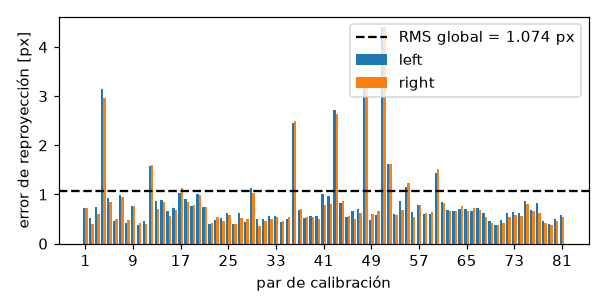
\includegraphics[width=\columnwidth]{00_error_por_vista.png}
  \caption{Error de reproyección por par de calibración (izquierda y
  derecha) y RMS global.}
  \label{fig:errvista}
\end{figure}

La Figura~\ref{fig:rect} compara un par de captura antes y después de
rectificar. En las imágenes originales un mismo punto del tablero aparece en
filas distintas; tras rectificar, los puntos homólogos quedan sobre las
mismas líneas horizontales.

\begin{figure*}[t]
  \centering
  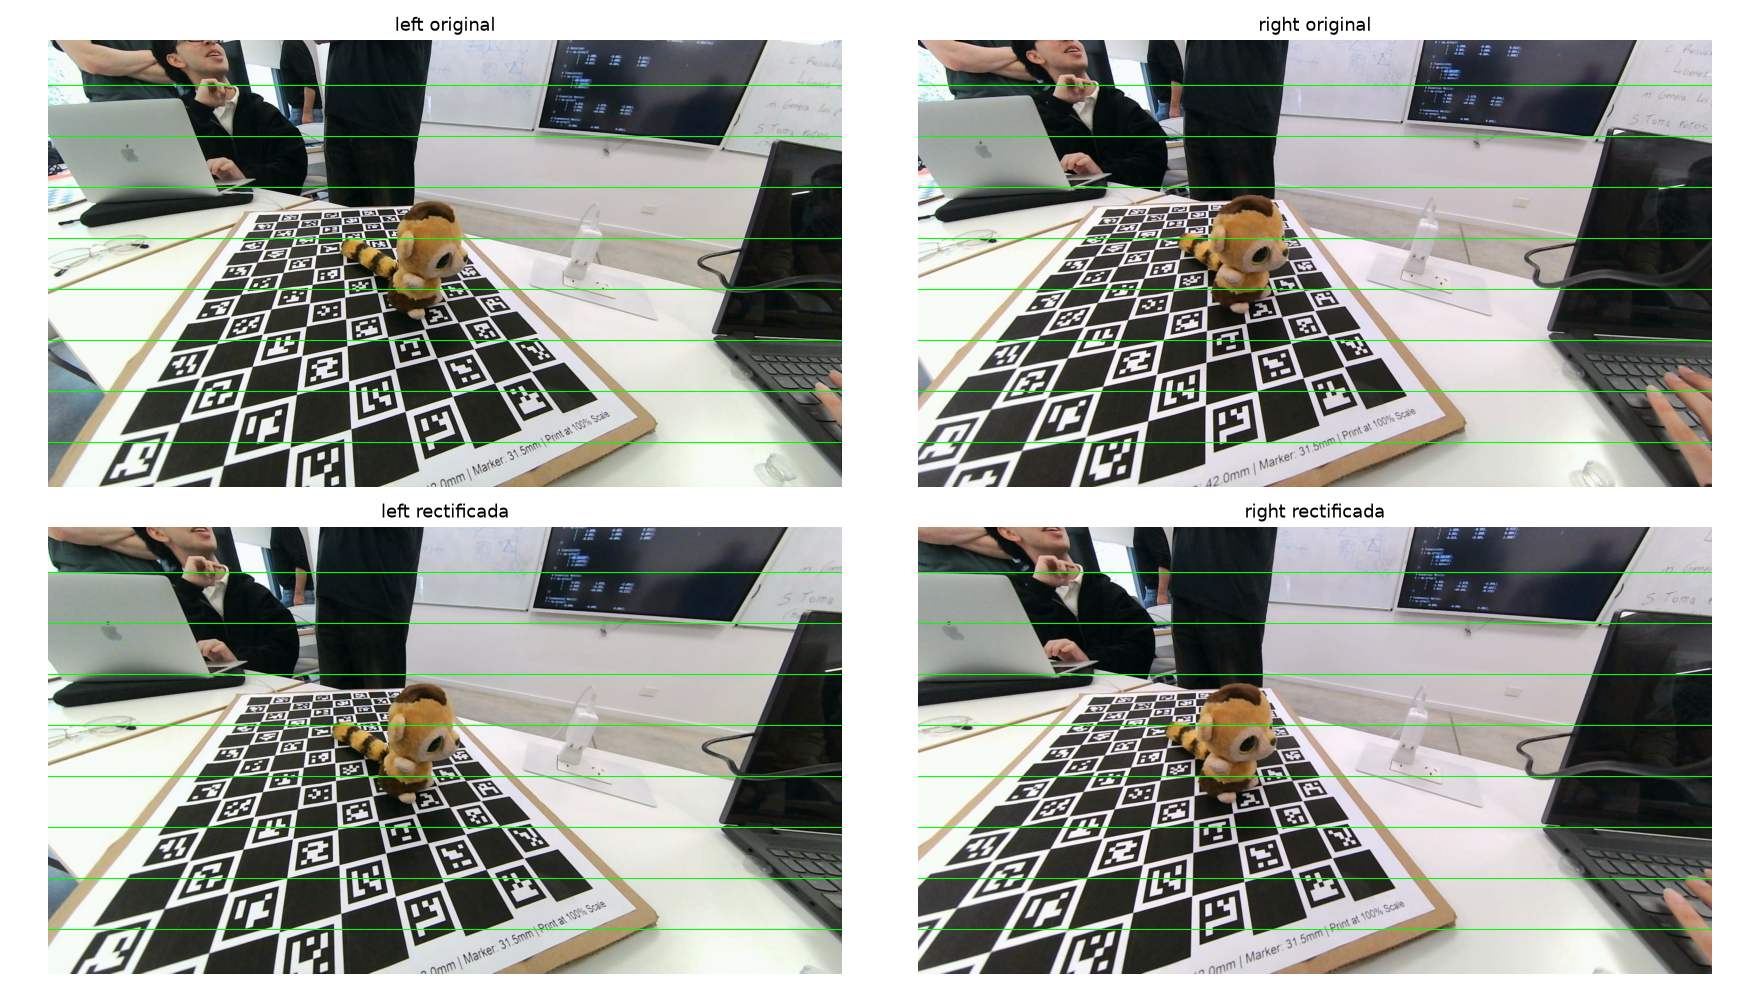
\includegraphics[width=0.78\textwidth]{02_rectificacion_captura.png}
  \caption{Par de captura original (arriba) y rectificado (abajo). Las
  líneas verdes horizontales permiten comparar la fila de los puntos
  homólogos.}
  \label{fig:rect}
\end{figure*}

\subsection{Disparidad}

La Figura~\ref{fig:disp} compara SGBM y CREStereo sobre el mismo par
rectificado, con la misma escala de colores. SGBM obtiene disparidad válida en
el 54\% de los píxeles, con huecos grandes en las zonas blancas del tablero y
de la mesa y mucho ruido en el fondo. CREStereo da un mapa denso (100\% de
píxeles) y suave, en el que el peluche se separa nítidamente del tablero. Las
disparidades sobre el objeto, de entre 125 y 150~px, corresponden según la
ecuación~\eqref{eq:depth} a distancias de 25 a 30~cm.

\begin{figure*}[t]
  \centering
  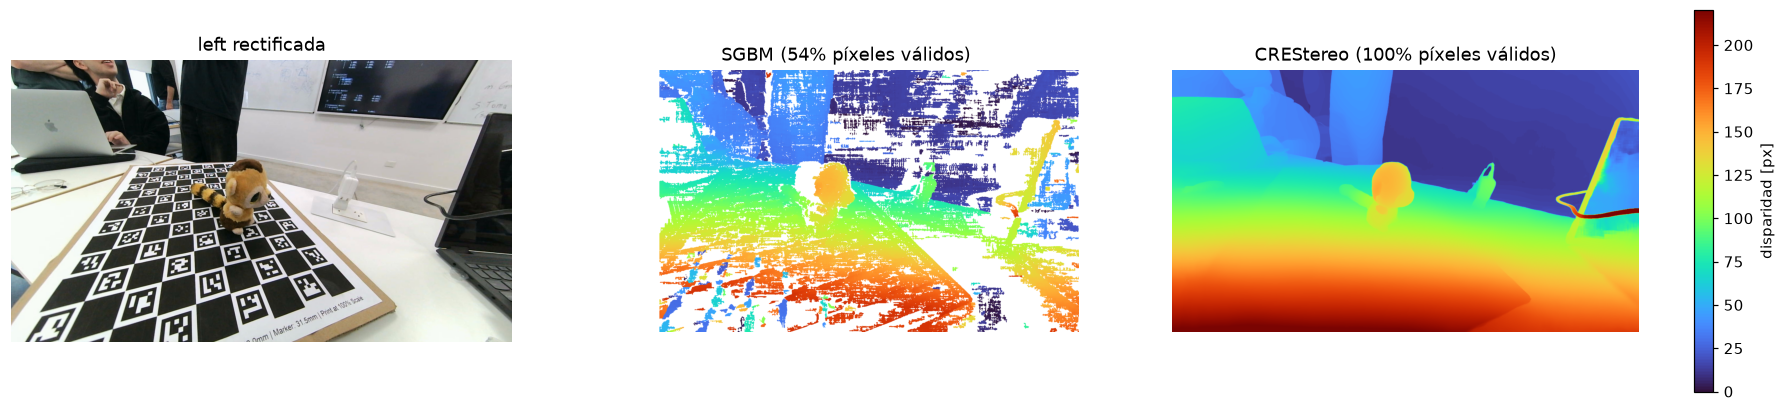
\includegraphics[width=\textwidth]{03b_sgbm_vs_crestereo.png}
  \caption{Imagen izquierda rectificada y disparidad obtenida con SGBM y con
  CREStereo (misma escala de colores; en blanco, píxeles sin disparidad
  válida).}
  \label{fig:disp}
\end{figure*}

\begin{figure*}[t]
  \centering
  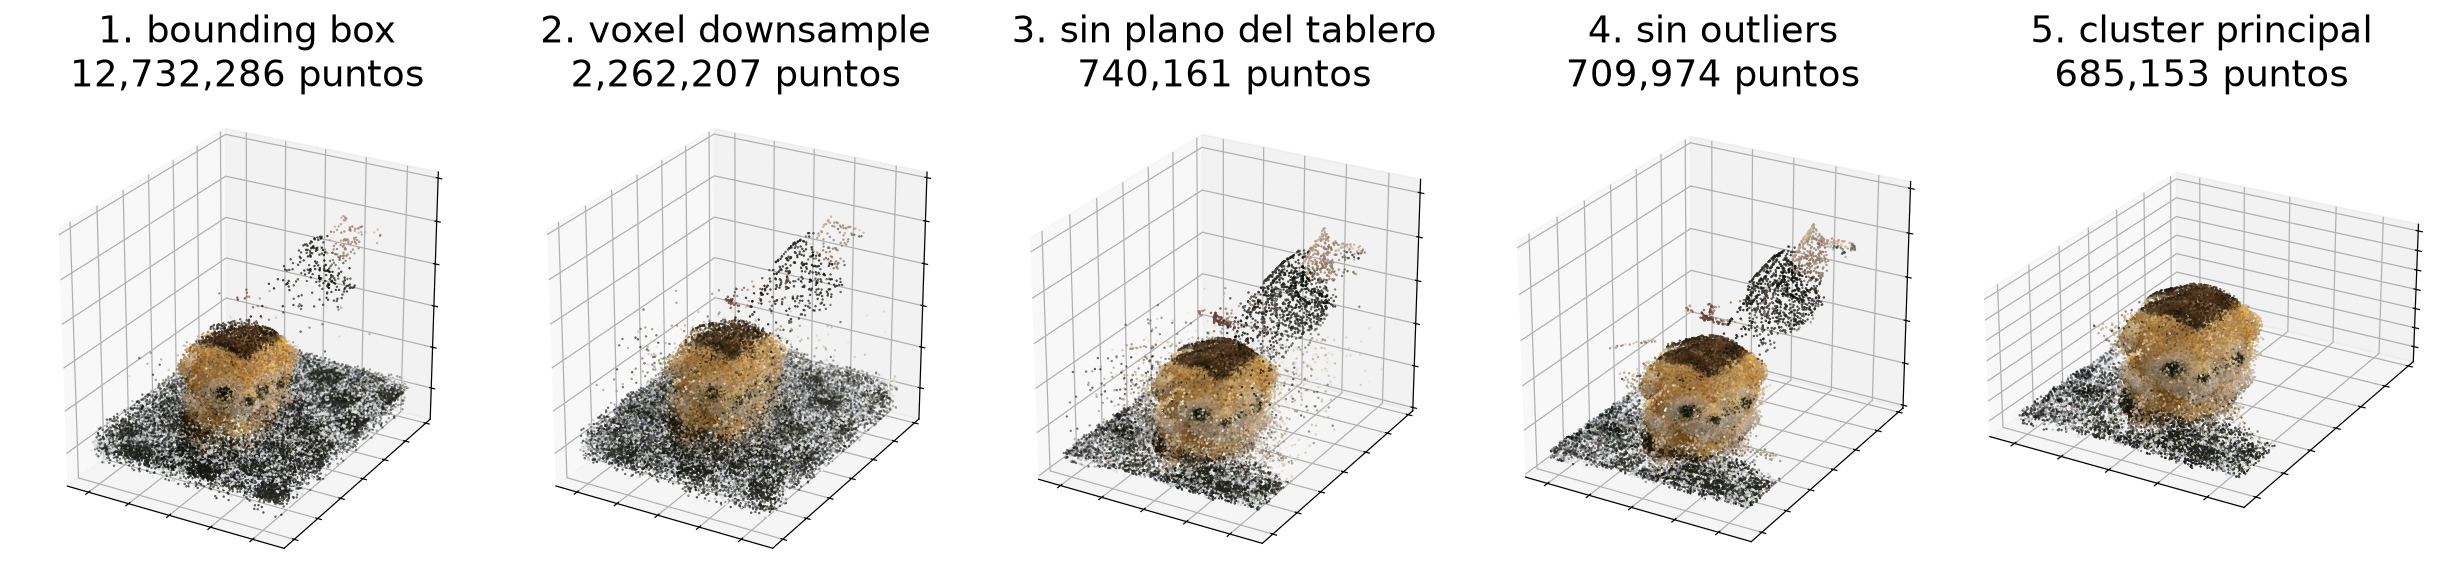
\includegraphics[width=\textwidth]{06a_etapas_optimizacion.png}
  \caption{Nube después de cada etapa de optimización, con la cantidad de
  puntos sobrevivientes.}
  \label{fig:etapas}
\end{figure*}

\begin{figure*}[t]
  \centering
  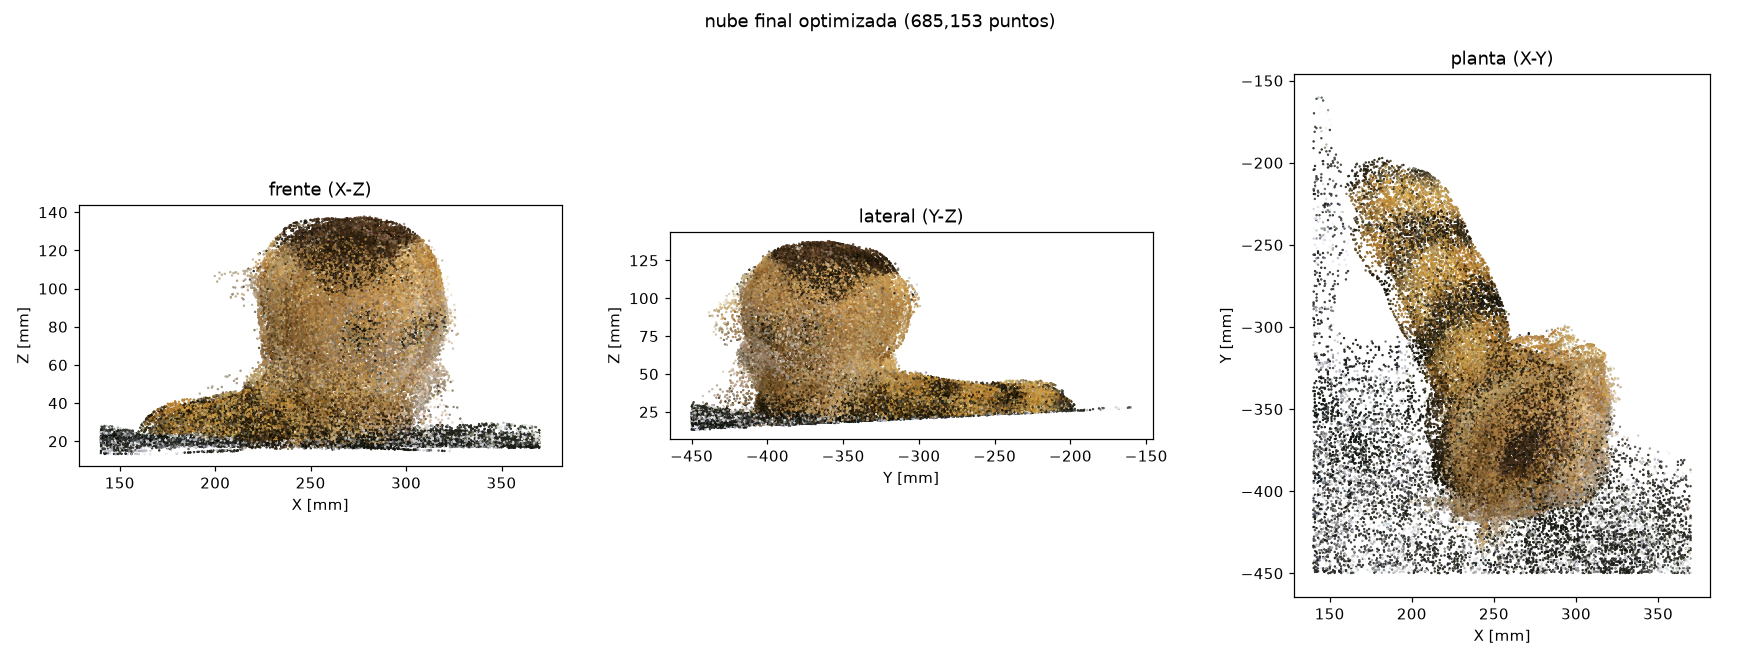
\includegraphics[width=0.9\textwidth]{06_nube_final.png}
  \caption{Nube final optimizada: vista frontal, lateral y en planta
  (coordenadas del mundo, en mm).}
  \label{fig:final}
\end{figure*}

\subsection{Pose de las cámaras}

Se estimó la pose con PnP en las 58 capturas, usando entre 67 y 279
correspondencias por vista (mediana 175). El error de reproyección de PnP
(Figura~\ref{fig:pnp}) fue de 1.52 a 4.29~px, con mediana de 2.47~px. La
Figura~\ref{fig:poses} muestra las cámaras estimadas sobre la escena: forman
una órbita alrededor del peluche, a entre 21 y 45~cm de él y a alturas de 9
a 42~cm sobre el tablero, lo que coincide con el recorrido realizado al
capturar.

\begin{figure}[t]
  \centering
  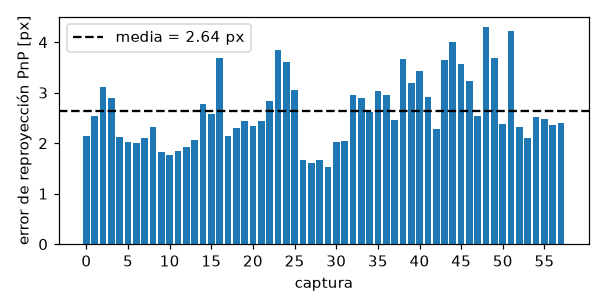
\includegraphics[width=\columnwidth]{04b_error_pnp_por_captura.png}
  \caption{Error de reproyección de PnP en cada captura.}
  \label{fig:pnp}
\end{figure}

\begin{figure}[t]
  \centering
  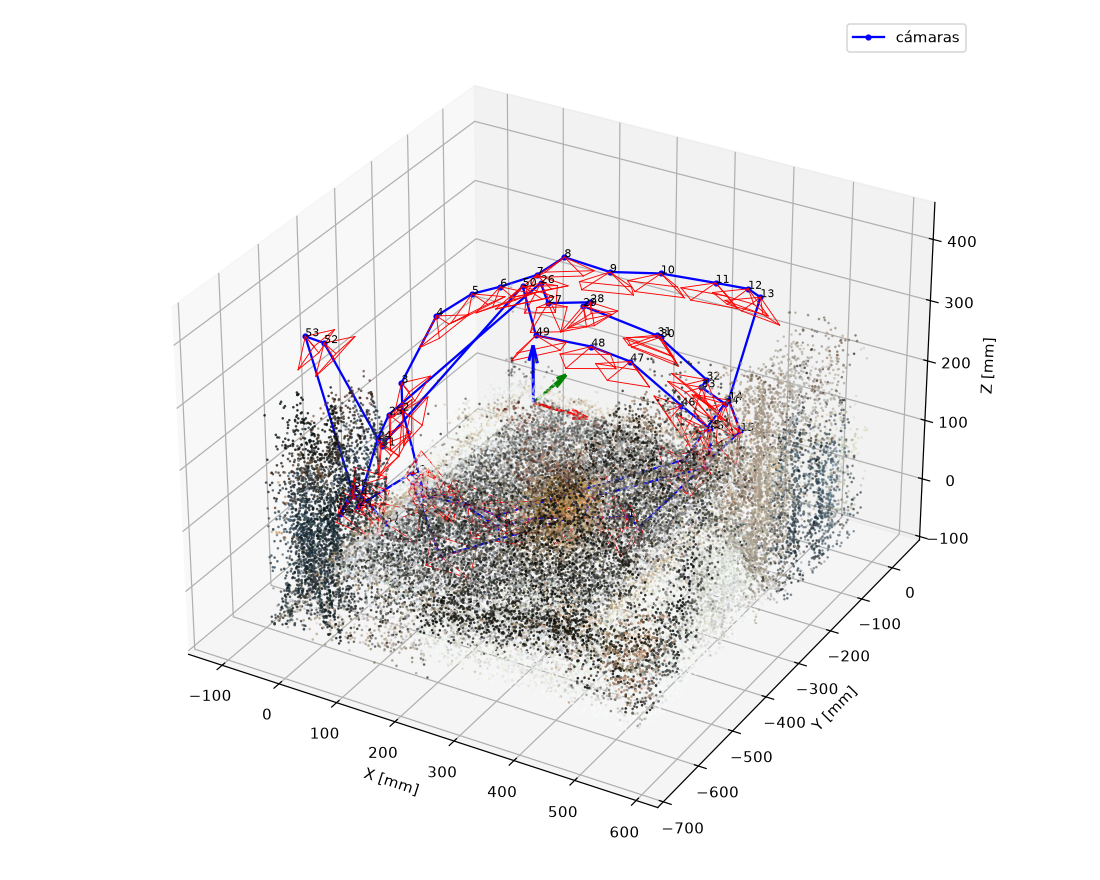
\includegraphics[width=\columnwidth]{05_poses_camaras.png}
  \caption{Poses de cámara estimadas (pirámides rojas, numeradas en orden
  de captura) sobre la escena fusionada, con los ejes del mundo en el
  origen del ChArUco ($X$ rojo, $Y$ verde, $Z$ azul hacia arriba).}
  \label{fig:poses}
\end{figure}

\subsection{Fusión y optimización}

La Tabla~\ref{tab:etapas} muestra la cantidad de puntos después de cada
etapa, y la Figura~\ref{fig:etapas}, la nube resultante. La caja se queda con
el 13\% de la escena, y el submuestreo con vóxeles de 1~mm reduce la nube
5.6 veces, ya que muchas vistas solapadas ven las mismas superficies. La
remoción del plano elimina la mayor parte del tablero. El filtro estadístico
y DBSCAN eliminan, respectivamente, puntos aislados y un objeto de la mesa
que había quedado dentro de la caja (visible arriba a la derecha en las
etapas 1 a 4). La nube final tiene 685\,153 puntos y el archivo
\texttt{reconstruction.ply} pesa 18.5~MB, en el orden pedido.

\begin{table}[t]
  \centering
  \caption{Puntos sobrevivientes en cada etapa.}
  \label{tab:etapas}
  \begin{tabular}{@{}lrr@{}}
    \toprule
    Etapa & Puntos & \% del anterior \\
    \midrule
    Nube fusionada (58 vistas) & 100\,043\,139 & -- \\
    Caja (filtrado espacial)   & 12\,732\,286 & 12.7\% \\
    Vóxel 1~mm                 & 2\,262\,207  & 17.8\% \\
    Sin plano del tablero      & 740\,161     & 32.7\% \\
    Sin outliers estadísticos  & 709\,974     & 95.9\% \\
    Cluster principal (final)  & 685\,153     & 96.5\% \\
    \bottomrule
  \end{tabular}
\end{table}

La Figura~\ref{fig:final} muestra la nube final en tres proyecciones y la
Figura~\ref{fig:malla}, la malla obtenida por Poisson. Se reconocen la
cabeza, el cuerpo y la cola rayada apoyada sobre el tablero.

\begin{figure}[t]
  \centering
  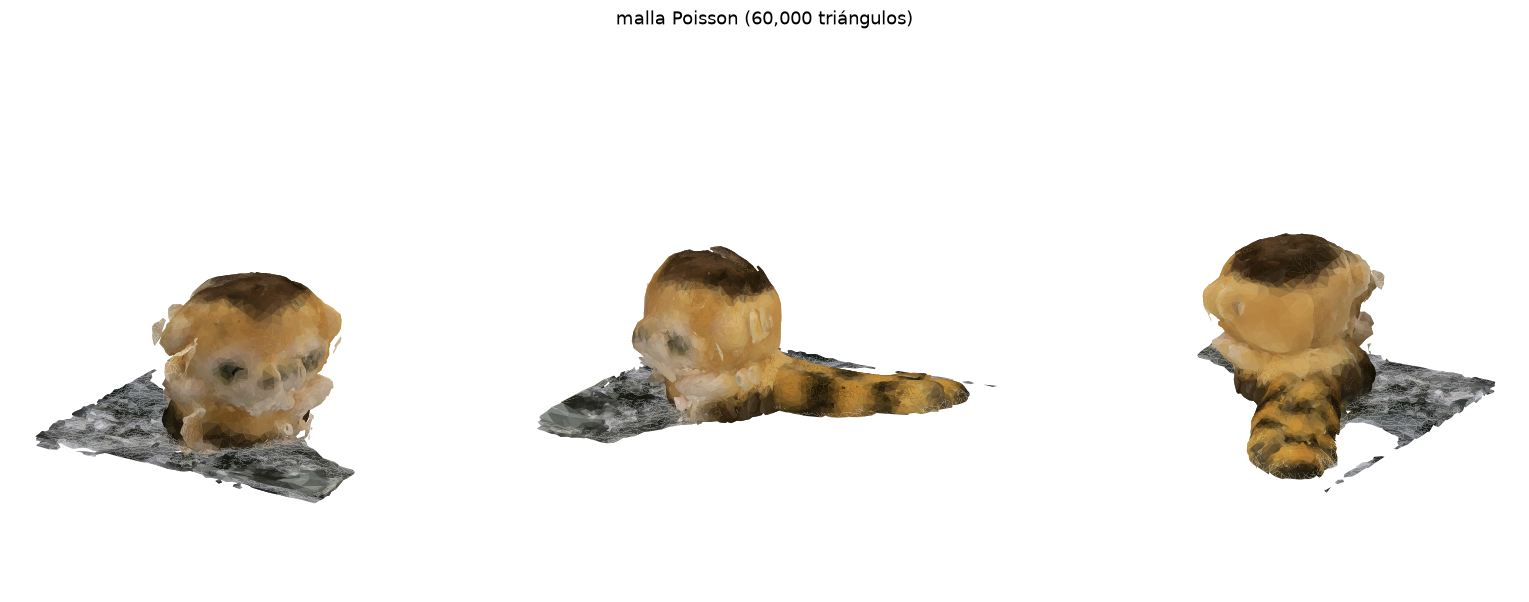
\includegraphics[width=\columnwidth, trim=0 60 0 147, clip]{07_malla_poisson.png}
  \caption{Malla obtenida por reconstrucción de Poisson, vista desde tres
  ángulos.}
  \label{fig:malla}
\end{figure}

\subsection{Medición métrica}

La Tabla~\ref{tab:medicion} resume las medidas. La altura del peluche sobre
el plano de apoyo es de \textbf{130.5~mm} (percentil 99.5; el punto más alto
está a 134.1~mm). Medido con regla, el peluche tiene una altura de
\alturareal~mm, lo que da un error relativo de \errorrel. El ancho y la
profundidad están sobreestimados por los restos del tablero que quedan junto
a la base (ver Discusión), por lo que se reportan solo como cota superior.

\begin{table}[t]
  \centering
  \caption{Dimensiones estimadas del peluche.}
  \label{tab:medicion}
  \begin{tabular}{@{}lr@{}}
    \toprule
    Medida & Valor [mm] \\
    \midrule
    Alto (sobre el plano, percentil 99.5) & \textbf{130.5} \\
    Alto (punto más alto)                  & 134.1 \\
    Ancho en $X$ (percentiles 0.5--99.5)   & 216.9$^\ast$ \\
    Profundidad en $Y$ (percentiles 0.5--99.5) & 238.9$^\ast$ \\
    \midrule
    Alto real (regla)                      & \alturareal \\
    \bottomrule
    \multicolumn{2}{@{}l}{\footnotesize $^\ast$ Incluyen restos del tablero junto a la base.}
  \end{tabular}
\end{table}

\subsection{Validación con el dataset de la cátedra}

Para separar los problemas del método de los de la captura, se corrió el
mismo pipeline sobre \texttt{stereo\_budha\_charuco} (21 capturas), con SGBM.
La calibración usó 20 de 21 pares (RMS 1.06~px, baseline 59.95~mm), y el
error de PnP fue de 0.90 a 1.80~px (mediana 1.11~px), menos de la mitad que en
el dataset propio. La nube final tiene 682\,042 puntos y el Buda mide
272.6~mm de alto.

% =====================================================================
\section{Discusión}
% =====================================================================

\subsection{Calidad de la calibración}

El RMS de 1.07~px es aceptable, pero está dominado por unos pocos pares: la
mediana por vista es de 0.66~px y solo cinco pares superan los 2~px. Lo más
probable es que esas imágenes tengan desenfoque por movimiento o que las dos
cámaras no las hayan capturado en el mismo instante. Descartarlas y volver a
calibrar bajaría el RMS sin perder cobertura, porque quedan 76 pares. Los
intrínsecos son muy parecidos a los del dataset de la cátedra
($f\approx600$~px, baseline de 60~mm), lo que es coherente con que se trata
del mismo modelo de cámara.

\subsection{Desalineamiento vertical residual}

El principal problema encontrado es que, después de rectificar, los puntos
homólogos entre izquierda y derecha (medidos con correspondencias SIFT) no
quedan exactamente en la misma fila: tienen un desalineamiento vertical de
$\pm$1--4~px, mientras que en el dataset del Buda es de unos 0.1~px. El
desalineamiento aparece también con los mapas de \texttt{calib-stereo} y
cambia de signo entre capturas, por lo que no se trata de un error fijo de
calibración. La explicación más probable es el movimiento de la cámara en la
mano durante cada toma: si los dos sensores no capturan exactamente al mismo
tiempo, la cámara se mueve entre una imagen y la otra y el par deja de
cumplir la geometría calibrada.

Esto explica varios resultados. SGBM busca la correspondencia solo sobre la
misma fila, por eso falla en la mitad de los píxeles, mientras que CREStereo
incluye una correlación con búsqueda local en 2D, pensada justamente para
pares con rectificación imperfecta, y tolera mejor el desalineamiento.
Además, cada nube local tiene un error de profundidad de $\pm$5--7\%. Este
error no es un sesgo de escala global: el cociente entre la profundidad
estéreo y la que da PnP en las esquinas del tablero tiene mediana 0.996.
Pero las nubes de distintas vistas no coinciden del todo, y por eso la cara
del peluche aparece borrosa o duplicada en la malla
(Figura~\ref{fig:malla}). El mayor error de PnP respecto del Buda (2.5 contra
1.1~px de mediana) es coherente con el mismo problema.

\subsection{El tablero reconstruido y la medición}

Por la misma razón, el tablero no se reconstruye como un plano sino como una
capa de 1 a 4~cm de espesor. El plano ajustado por RANSAC está inclinado
unos $3^\circ$ y queda unos 19~mm por encima del plano $Z=0$ que da PnP. Por
eso la altura se mide respecto del plano reconstruido y no respecto de
$Z=0$: como el peluche se apoya sobre el tablero reconstruido, ambos tienen el
mismo sesgo y la diferencia lo cancela. Si se midiera desde $Z=0$, la altura
quedaría inflada en unos 19~mm.

La capa gruesa del tablero también obliga a usar un margen de 15~mm al
remover el plano, y eso genera un compromiso: quedan restos del tablero junto
a la base, conectados al peluche (DBSCAN no puede separarlos), y a la vez se
pierde la parte inferior de la cola, que está apoyada y tiene apenas unos
2--3~cm de alto. Esos restos son los que inflan el ancho y la profundidad
(Figura~\ref{fig:final}, vista en planta), por lo que la medida confiable es
la altura.

\subsection{Posibles mejoras}

\begin{itemize}
  \item \textbf{Captura:} apoyar la cámara (trípode o superficie fija) en
        cada toma para eliminar el movimiento durante la captura, que es la
        causa principal de los errores observados.
  \item \textbf{Calibración:} descartar los pares con error por vista
        alto y volver a calibrar.
  \item \textbf{Registro entre vistas:} refinar la pose de cada nube con
        ICP (punto a plano) contra la nube acumulada, o alinear cada nube
        local al plano conocido del tablero antes de fusionar. Esto
        corregiría el desalineamiento de la cara y adelgazaría la capa del
        tablero, lo que permitiría usar un margen menor y conservar la cola
        completa.
  \item \textbf{Medición:} en lugar de extensiones en $X$ e $Y$, segmentar
        el objeto en la planta y medir con una caja orientada mínima,
        menos sensible a los restos del tablero.
\end{itemize}

% =====================================================================
\section{Conclusiones}
% =====================================================================

Se implementó un pipeline completo de reconstrucción 3D por estéreo
multivista, desde la calibración de la cámara hasta una nube de puntos
métrica del objeto, y se lo aplicó a un dataset propio de 58 pares. El
sistema se calibró con un RMS de 1.07~px y un baseline de 60.70~mm; la pose
se estimó con PnP sobre el ChArUco en todas las capturas, y la fusión y
optimización dieron una nube final de 685\,153 puntos en la que se reconoce
claramente el peluche. La altura estimada es de 130.5~mm, frente a
\alturareal~mm medidos con regla (error relativo de \errorrel).

Dos decisiones resultaron clave. La primera fue estimar la pose sobre la
imagen rectificada con $K_{\text{rect}}=P_1[:, :3]$, lo que deja la pose y
la nube local en el mismo sistema sin componer con $R_1$. La segunda fue
usar CREStereo en lugar de SGBM: con capturas imperfectas, la red da
disparidades densas donde SGBM deja la mitad de los píxeles sin valor.

La comparación con el dataset de la cátedra muestra que las limitaciones
observadas (cara duplicada, tablero grueso, ancho y profundidad inflados)
vienen principalmente de la captura y no del método: con pares bien
sincronizados el mismo pipeline produce una reconstrucción limpia y un
error de PnP de la mitad. Por eso la mejora más importante sería volver a
capturar con la cámara apoyada; ICP permitiría además corregir el registro
entre vistas que queda.

\end{document}
